\section{Funkce}

\subsection{Elementární funkce}

Elementární funkce jsou takové, které lze složit konečným počtem operací (sčítání, odčítání, násobení, dělení a skládání) z těchto funkcí: konstanta, obecná mocnina, exponenciála, logaritmus, sinus, kosinus, tangens, kontangens, arkussinus, arkuskosinus, arkustangens a arkuskotangens. 

Jiné funkce než elementární v kurzu prakticky nepotkáme. Je jich ale spousta. Příklady neelementárních funkcí si ukážeme, až budeme vybaveni mocnými nástroji, jako je určitý integrál.

\subsection{Definiční obor}

Definiční obor $D(f)$ (též $D_f$) je množina takových čísel, pro která je funkce $f$ definována.

Při určování definičního oboru elementárních funkcí se v podstatě můžeme řídit jednoduchými zásadami.

\begin{enumerate}
    \item Nesmíme dělit nulou.
    \item Sudé odmocniny jsou definované pouze pro nezáporná čísla.
    \item Logaritmus je definovaný pouze pro kladná čísla.
    \item Speciální pozornost si zaslouží funkce $\tan$, $\cot$, $\arcsin$ a $\arccos$.
\end{enumerate}

Kompletní přehled dává tabulka.

\begin{table}[H]
    \centering
    \begin{tabular}{||c|c|c||}
        \hline \hline
        funkce & definiční obor & obor hodnot \\
        \hline
        $x^k$, $k$ je sudé              & $\R$          & $[0, \infty)$ \\ 
        $x^k$, $k$ je liché             & $\R$          & $\R$ \\ 
        $\sqrt[k]{x}$, $k$ je sudé      & $[0, \infty)$ & $[0, \infty)$ \\
        $\sqrt[k]{x}$, $k$ je liché     & $\R$          & $\R$ \\
        $x^\alpha$, $\alpha \in \R$     & $(0, \infty)$ & $(0, \infty)$ \\
        $e^x$                           & $\R$          & $(0, \infty)$ \\
        $a^x$                           & $\R$          & $(0, \infty)$ \\
        $\log x$                        & $(0, \infty)$ & $\R$ \\
        $\sin x$, $\cos x$              & $\R$          & $[0,1]$ \\
        $\tan x$                        & $\R \setminus \set{\pi/2 + k \pi, k \in \Z}$ & $\R$ \\
        $\cot x$                        & $\R \setminus \set{k \pi, k \in \Z}$  & $\R$ \\
        $\arcsin x$                     & $[-1,1]$      & $[-\frac{\pi}{2}, \frac{\pi}{2}]$ \\
        $\arccos x$                     & $[-1,1]$      & $[0,\pi]$ \\
        $\arctan x$                     & $\R$          & $(-\frac{\pi}{2}, \frac{\pi}{2})$ \\
        $\arccot x$                     & $\R$          & $(0,\pi)$ \\
         \hline \hline
    \end{tabular}
    
\end{table}

\subsection{Růst a pokles funkce}
O funkci řekneme, že je \begin{itemize}
    \item \textbf{rostoucí} na intervalu $I$, jestliže pro všechna $x,y \in I$ splňující $x<y$ platí $f(x) < f(y)$,
    \item \textbf{klesající} na intervalu $I$, jestliže pro všechna $x,y \in I$ splňující $x<y$ platí $f(x) < f(y)$,
    \item \textbf{neklesající} na intervalu $I$, jestliže pro všechna $x,y \in I$ splňující $x<y$ platí $f(x) \leq f(y)$,
    \item \textbf{nerostoucí} na intervalu $I$, jestliže pro všechna $x,y \in I$ splňující $x<y$ platí $f(x) \geq f(y)$,
    \item \textbf{konstantní} na intervalu $I$, jestliže pro všechna $x,y \in I$ splňující $x<y$ platí $f(x) = f(y)$,
    \item \textbf{monotónní} na intervalu $I$, jestliže je na něm neklesající, anebo nerostoucí.
\end{itemize}

\begin{figure}[H]
    \centering
    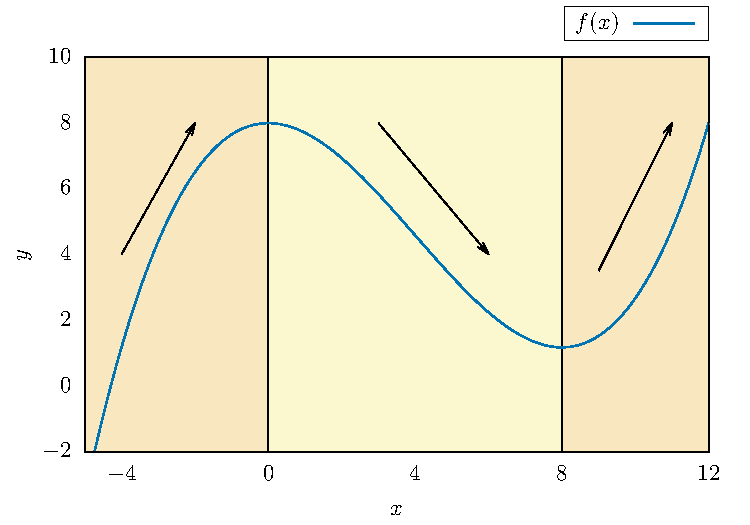
\includegraphics[scale = 0.7]{Gnuplot/Figures/funkce-rostouci-klesajici-obr.pdf}
    \caption{Ilustrace pojmu rostoucí a klesající funkce. Na oranžové oblasti je $f(x)$ rostoucí, na žluté oblasti je $f(x)$ klesající.}
\end{figure}

\begin{remark}
    Pokud mluvíme o růstu nebo poklesu funkce, je vždy nutné uvést, na jakém intervalu se pohybujeme. Důležitost je vidět na následujícím příkladu.

    \begin{figure}[H]
        \centering
        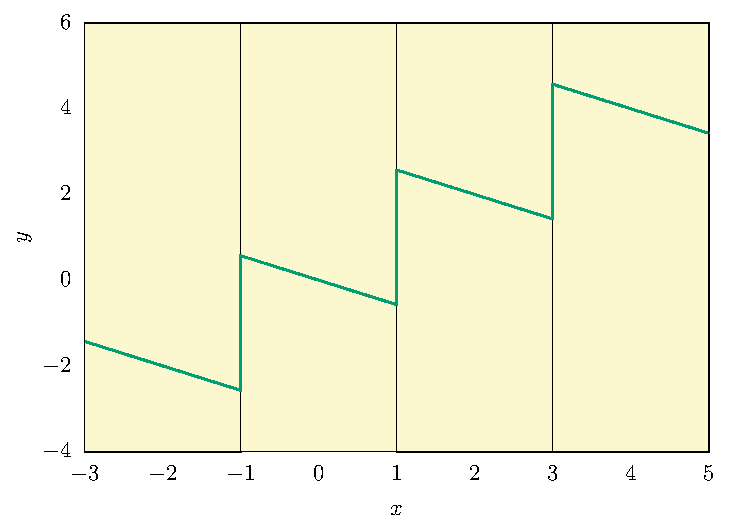
\includegraphics[scale = 0.7]{Gnuplot/Figures/periodicka-klesajici.pdf}
        \caption{Příklad funkce, která je klesající na každém intervalu $(2p-1,2p+1)$, $p \in \Z$, ale není klesající na celém $\R$ (nesplňuje definici klesající funkce - stačí porovnat dva body v oddělených intervalech). Dokonce se jeví jako \uv{globálně rostoucí}, ale s takovým pojmem nepracujeme. Všimněme si, že funkce je v krajních bodech intervalů nespojitá.}
    \end{figure}

\end{remark}

\begin{remark}
    V některé literatuře se o různých křivkách mluví jako o \uv{rostoucích zleva doprava} nebo \uv{klesajících zprava doleva} a podobně. Matematická terminologie vždy pracuje s tím, co se děje s hodnotami $f(x)$ \underline{při rostoucích $x$} - tedy vždy \uv{zleva doprava}, chcete-li. Podobně se někdy říká o klesajících funkcích $y(x)$, že \uv{$y$ je nepřímo úměrné $x$}. Ale matematická terminologie říká, že pouze funkce $y(x)=C/x$ je nepřímá úměrnost, žádná jiná funkce toto nesplňuje.

    \begin{figure}[H]
        \centering
        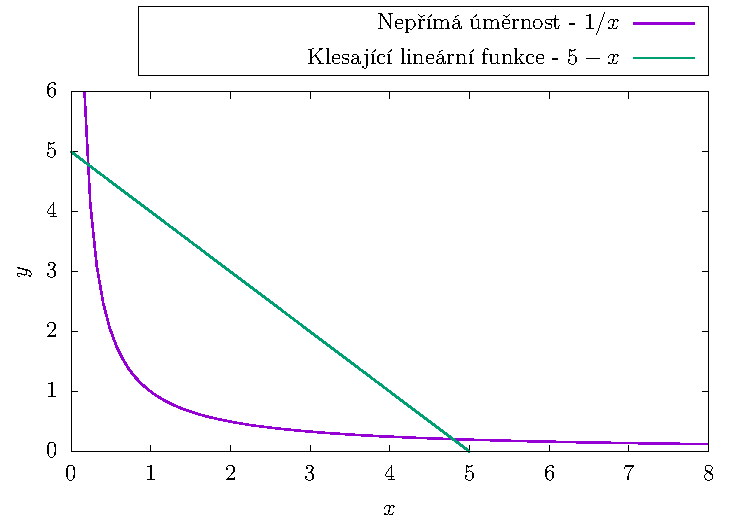
\includegraphics[scale = 0.7]{Gnuplot/Figures/neprima-umernost.pdf}
        \caption{Ilustrace často nesprávně použitého termínu \uv{nepřímá úměrnost}. Pouze funkce typu $C/x$ jsou nepřímé úměrnosti.}
    \end{figure}
\end{remark}

\subsection{Další charakteristiky funkce}

O funkci $f(x)$ říkáme, že je \begin{itemize}
    \item \textbf{prostá} na intervalu $I$, jestliže pro všechna $x,y \in I$ splňující $x \neq y$ platí $f(x) \neq f(y)$ (\uv{každému $x$ přísluší jiná hodnota $f(x)$}),
    \item \textbf{omezená shora}, jestliže existuje konečné číslo $K$ takové, že pro všechna $x \in D(f)$ platí $f(x) \leq K$,
    \item \textbf{omezená zdola}, jestliže existuje konečné číslo $K$ takové, že pro všechna $x \in D(f)$ platí $f(x) \geq K$,
    \item \textbf{omezená}, jestliže je omezená shora i zdola.
\end{itemize}

Jestliže je funkce $f$ prostá na intervalu $I$, pak k ní existuje \textbf{inverzní funkce}, kterou označujeme $f^{-1}$.

\begin{example}
    Funkce $x^2$ je prostá na intervalu $(-\infty, 0]$ a na intervalu $[0,+\infty)$. Není prostá na $\R$, protože $(-2)^2 = 4 = (+2)^2$.

    Na intervalu $[0,\infty)$ k ní existuje inverzní funkce $\sqrt{x}$. Na intervalu $(-\infty,0]$ k ní existuje inverzní funkce $\sqrt{-x}$.
\end{example}



\subsection{Příklady na definiční obor}

\begin{example}
    Určíme definiční obor funkce \begin{align*}
        R(x) = \frac{x^2-1}{(x+1)(x-4)(x^2 + 4x - 5)} \:.
    \end{align*}

    Řešení: První pravidlo nám říká, že nesmíme dělit nulou. Musíme tedy najít všechna $x$ taková, že je jmenovatel zZákladní vlastnosti funkcílomku nulový: \begin{align*}
        (x+1)(x-4)(x^2 + 4x - 5) = 0 \:.
    \end{align*}
    Součin čísel (nebo výrazů, závorek) je nulový tehdy a jen tehdy, když je jedno z čísel nulové. Každou závorku tedy řešíme zvlášť:
    \begin{align*}
        x+1 =& 0 \Longrightarrow x = -1 \:, \\
        x-4 =& 0 \Longrightarrow x = 4 \:, \\
        x^2 + 4x - 5 =& 0 \Longrightarrow \frac{-4 \pm \sqrt{16+20}}{2} = - 2 \pm 3 \:, \: x = -5, 1 \:.
    \end{align*}
    Tato řešení jsou body, které musíme z definičního oboru vyloučit. Tedy \begin{align*}
        \boxed{D(R) = \R \setminus \set{-5,-1,1,4} }\:.
    \end{align*}
    Poznámka: někdo by snad mohl postupovat tak, že by čitatel rovněž převedl na součin závorek: $x^2-1 = (x-1)(x+1)$. Jmenovatel lze též převést na součin: $x^2+4x-5 = (x+5)(x-1)$. Postupoval by tedy krácením:
    \begin{align*}
        R(x) = \frac{(x-1)(x+1)}{(x+1)(x-4)(x+5)(x-1)} \overset{?}{=} \frac{1}{(x+1)(x-4)} \:.
    \end{align*}
    Výraz na levé straně má jiný definiční obor: $\R \setminus \set{-1,4} \neq D(R)$.
    \textbf{Číselné hodnoty výrazů napravo a nalevo jsou stejné, ale definiční obor výrazů je různý!} Poučení tedy je: nejdříve nalezneme definiční obor a pak můžeme krátit.
\end{example}

\begin{example}
    Ještě jednou upozorníme na stejný případ: funkce $f(x) = \frac{x}{x}$ odpovídá konstantní funkci $g(x) = 1$, s tím rozdílem, že do $f$ nelze dosadit nulu. Takže \begin{align*}
        D(f) = \R \setminus \set{0} \neq \R = D(g) \:.
    \end{align*}
    
\end{example}

\begin{example}
    Určíme definiční obor funkce \begin{align*}
        h(x) = \sqrt{ \frac{\log (x-2)}{x-4}}
    \end{align*}

    Řešení: 1. pravidlo nám vyloučí bod $x=4$. 
    Dále nám 3. pravidlo říká, že do $\log$ můžeme dosadit pouze kladná čísla, takže musí platit $x-2>0$. To odpovídá hodnotám $x \in (2, \infty)$. 
    Konečně nám 2. pravidlo říká, že musí být výraz pod odmocninou nezáporný, musíme tedy řešit nerovnici \begin{align*}
        \frac{\log (x-2)}{x-4} \geq 0 \:.
    \end{align*}
    Nejprve vyřešíme případ, kdy platí rovnost.
    \begin{align*}
        \log (x-2) = 0 \Longrightarrow x-2 = 1 \Longrightarrow x = 3 \:.
    \end{align*}
    
    Nyní vyřešíme případ nerovnosti. Podíl dvou čísel je větší než nula právě tehdy, když jsou obě čísla kladná anebo obě čísla záporná (samozřejmě \uv{minus krát minus je plus}). Stačí tedy řešit podmínky:
    \begin{align*}
        \left [\log (x-2) > 0 \right] \bigwedge \left[ x-4 > 0\right] \Longrightarrow [x \in (3,\infty)] \bigwedge [x \in (4, \infty)] \Longrightarrow x \in (4, \infty) \:, \\
        \left [\log (x-2) < 0 \right] \bigwedge \left[ x-4 < 0\right] \Longrightarrow [x \in (2,3)] \bigwedge [x \in (-\infty, 4)] \Longrightarrow x \in (2,3) \:.
    \end{align*}
    Celkově máme \begin{align*}
        \boxed{ D(h) = (2,3) \cup \set{3} \cup (4,\infty) = (2,3] \cup (4,\infty) } \:.
    \end{align*}
\end{example}

\begin{example}
    Určíme definiční obor funkce \begin{align*}
        P(x) = \frac{\arcsin (x-1)}{x^x} \:.
    \end{align*}

    Řešení: jmenovatel vyloučí bod nula. Dále, definiční obor funkce $\arcsin$ je $[-1,1]$, tedy $ -1 \geq x-1 \geq 1$, takže $x \in [0,2]$. 
    Nyní se podívejme na funkci ve jmenovateli. Tu můžeme přepsat \begin{align*}
        x^x = \left( e^{\log x} \right) = e^{x \log x} \:,
    \end{align*}
    takže se v ní objeví logaritmus a vidíme, že $x \in (0, \infty)$.
    Celkově \begin{align*}
        \boxed{ D(P) = [0,2] \cap (0, \infty) = (0,2] } \:.
    \end{align*}

\end{example}

\begin{example}
    Určíme definiční obor funkce 
    \begin{align*}
        m(t) = \tan (\sqrt{t+1}) \:.
    \end{align*}

    Řešení: odmocnina dává podmínku $t \in [-1,\infty)$. Dále platí $\tan x = \frac{\sin x}{\cos x} $, takže $\tan (\sqrt {t+1}) = \frac{\sin (\sqrt {t+1})}{\cos (\sqrt {t+1})}$. Protože nesmíme dělit nulou, musíme najít body \begin{align*}
        \cos (\sqrt{t+1}) = 0 \:.
    \end{align*}
    Substitucí $\sqrt{t+1} = u$ dostáváme podmínku $\cos u =0$, která odpovídá bodům $u = \frac{\pi}{2} + k \pi \:, k \in \Z$. Odtud máme \begin{align*}
        \sqrt{t+1} = \frac{\pi}{2} + k \pi \:.
    \end{align*}
    Nyní musíme vyjádřit $t$, což uděláme prostým umocněním a odečtením jedničky:
    \begin{align*}
        t =  \left( \frac{\pi}{2} + k \pi \right)^2 - 1 = \frac{\pi^2}{4} + 2 \cdot k \pi \cdot \frac{\pi}{2} + k^2 \pi^2 - 1 = k^2 \pi^2 + k \pi^2 + \frac{\pi^2}{4} - 1 \:.
    \end{align*}
    Definiční obor je tedy \begin{align*}
        D(m) = \set{t : t \geq -1, t \neq k^2 \pi^2 + k \pi^2 + \frac{\pi^2}{4} - 1, \: k \in \Z} \:.
    \end{align*}
\end{example}

\begin{example}
    Určíme definiční obor funkce \begin{align*}
        g(x) = \frac{\sin^3 x + 4^{-x}}{\sqrt{|2x-1|-|x+1|-3}} \:.
    \end{align*}
    Funkce v čitateli mají definiční obor $\R$. Musíme tedy zařídit, aby odmocnina ve jmenovateli byla dobře definovaná a aby byla nenulová, to znamená zajistit \begin{align*}
        |2x-1|-|x+1|-3 > 0 \:.
    \end{align*}

    Nerovnice s absolutní hodnotou se řeší pomocí tabulek. Nejprve najdeme body, kdy je absolutní hodnota nulová. V našem případě to jsou body $2x-1 = 0 \Rightarrow x=1/2$ a $x+1=0 \Rightarrow x=-1$. Nyní stačí využít toho, že $|x| = +x$ pro $x>0$ a $|x| = -x$ pro $x<0$.

    \begin{table}[H]
        \centering
        \begin{tabular}{c||c|c|c}
            interval & $(-\infty,-1)$ & $(-1,1/2)$ & $(1/2, +\infty)$ \\
            \hline
            $|2x-1|$ & $-2x+1$ & $-2x+1$ & $+2x-1$ \\
            \hline
            $|x+1|$ & $-x-1$ & $+x+1$ & $+x+1$ \\
            \hline \hline
            $|2x-1|-|x+1|-3$ & $(-2x+1)-(-x-1)-3$ & $(-2x+1)-(+x+1)-3$ & $(+2x-1)-(+x+1)-3$ \\
            \hline
            po úpravě & $-x-1$ & $ -3x - 3$ & $x-5$   
        \end{tabular}
    \end{table}
    Nyní musíme vyřešit tři nerovnice \begin{align*}
        -x-1>0 \:, \quad -3x -3 >0 \:, \quad x-5 > 0 
    \end{align*}
    a podívat se, jestli spadají do zadaného intervalu.

    První rovnice odpovídá $x \in (-\infty,-1)$, což je v souladu s intervalem.
    Druhá rovnice odpovídá $x \in (-\infty,-1)$, který už není v souladu s intervalem.
    Třetí rovnice odpovídá $x \in (5, \infty)$, což je v souladu s intervalem.

    Celkově dostáváme 
    \begin{align*}
        \boxed{ D(g) = (-\infty, -1) \cup (5, \infty) } \:.
    \end{align*}
\end{example}
